%%%%%%%%%%%%%%%%%%%%%%%%%%%%%%
% Modèle type de présentation
%%%%%%%%%%%%%%%%%%%%%%%%%%%%%%

%-----------
% Préambule
%-----------

% faire tourner avec xelatex file.tex

% Type de document et encodage :
\documentclass[11pt]{beamer}
\usepackage[utf8x]{inputenc}
\usetheme[progressbar=foot,numbering=none]{metropolis}
%% \hypersetup{pdfpagemode=FullScreen}

% Langue :
\usepackage[french]{babel}

% Mise en forme :
\setbeamertemplate{caption}{\raggedright\insertcaption\par} % figure
\usepackage{enumitem} % listes
\usepackage{graphicx} % images
\usepackage{media9} % videos
\definecolor{foret}{rgb}{0.0353,0.3216,0.1569} % vert forêt
\setbeamercolor{title separator}{fg=celadon} % couleur séparateur de titre
\setbeamercolor{progress bar}{fg=celadon} % couleur barre de progression
 %\definecolor{MyBackground}{RGB}{255,241,167}
\usepackage{animate} %need the animate.sty file
\setbeamercolor{background canvas}{bg=white}
\definecolor{darkterracotta}{rgb}{0.8, 0.31, 0.36}
\definecolor{aquamarine}{rgb}{0.5, 1.0, 0.83}
\definecolor{carminepink}{rgb}{0.92, 0.3, 0.26}
\definecolor{burntsienna}{rgb}{0.91, 0.45, 0.32}
\definecolor{celadon}{rgb}{0.67, 0.88, 0.69}
\definecolor{caribbeangreen}{rgb}{0.0, 0.8, 0.6}
\definecolor{bittersweet}{rgb}{1.0, 0.44, 0.37}
\setbeamercolor{normal text}{fg=black, bg=black}
\newcommand{\ig}{\includegraphics}
\makeatletter
\setlength{\metropolis@titleseparator@linewidth}{1pt} % épaisseur séparateur de titre
\setlength{\metropolis@progressonsectionpage@linewidth}{2pt} % épaisseur barre de progression (section)
\setlength{\metropolis@progressinheadfoot@linewidth}{3pt} % épaisseur barre de progression (bas de page)
\makeatother

	
                  
\begin{document}


\title{
\includegraphics[scale=0.10]{logoincc.jpg}  
\includegraphics[scale=0.3]{ed3c.png} 
\includegraphics[scale=0.05]{logouniv.jpg}  
\includegraphics[scale=0.03]{logocnrs.png} \\
      
  {\textcolor{black}{Studying the aquisition of mathematical concepts through the generalization of a geometrical primitive from euclidean to non-euclidean geometry}}\\
  
  {\small {\textcolor{black}{Charlotte Barot, sous la direction de  V\'{e}ronique Izard}}\\
    {\textcolor{black}Comité : Valéria Giardino et Jérôme Sackur }}\\
        
     }

  
        \begin{frame}
          \titlepage
        \end{frame}



        \section{Introduction}

        \begin{frame}

          \centering
          
        How do we learn new mathematical concepts ?

        \end{frame}


        \begin{frame}

          Studying the change of paradigm in geometry, from euclidean geometry to a more general geometry, using a fundamental concept : straight line


        \end{frame}


        

        \begin{frame}
          Why non euclidean geometry ?
                    
          For almost 2000 years, euclidean geometry was considered as the natural geometry (Plato, Descartes, Kant)

          Euclidean geometry is the most easy to conceive for humans (Spelke, Lee and Izard 2010; Izard, Pica and Dehaene 2011)          
          
          Non euclidean systems are late in the history of humanity

          Emerged in a formal way, from a failed attempt to prove its contradiction
          
          Some of its models contradicts basic postulates of euclidean geometry, notably the fact that there always exist a parallel line to another one


        \end{frame}


        \begin{frame}

          Euclidean geometry is historically considered as the most easy to conceive (Spelke, Lee and Izard 2010 )

          Is it the case for a fundamental concept such as straight line ? Does it reflects the euclidean intuitions?

        \end{frame}
        
        \begin{frame}


          Straight line: a fundamental concept of euclidean geometry. Non primitive, used as a basic concept for more complex definitions, and hard to define without circularity

          Euclid's definition : \textit{A line is a length without width, and a straight line is a line equally placed between its points}

        \end{frame}

        \begin{frame}

           The generalization of straight line to curved surfaces is the geodesic

          Starting from a given point on a surface, it is a path which has a constant direction and never turns

        \end{frame}
        

        \begin{frame}

          
         

          
          \hfill
          
          \begin{tabular}{c|c|c}



                  &   Straight line   & Geodesic  \\

            \hline
            
             Constant direction  &  X  &  X   \\

             Shortest path       &  X  &      \\

             Infinite              &  X  &      \\

             Planar            &  X  &      \\


          \end{tabular}

          \hfill
          
          Straight line is a singular case of geodesic: a geodesic may intersect itself, be finite, and of non null curvature degree

        \end{frame}
       

        \section{Plan of the thesis}
        
        \begin{frame}
          
         \textcolor{bittersweet}{Intuition:} does euclidean intuition shape the representation of straight line? If yes, is it possible to change the initial intuition, or do humans just learn heuristics and methods to answer correctly to specific problems? (Article in preparation, data in collection)
          
         \textcolor{bittersweet}{ Dynamic of learning and metacognition:}
          is there a specific metacognitive signature associated to a new learning situation? (One article submitted, an online replication planned) 
          

          \textcolor{bittersweet}{Novelty of concept}: do participants build a new representation when learning or do they just use a new representation in addition, if any? (Article in preparation, ongoing analyses) 

        \end{frame}

             
        %% \begin{frame}

          

        %%   \normalsize
          
        %%   \textcolor{white}{}

        %%   \textcolor{white}{}


        %%   \textcolor{white}{}

        %%   \textcolor{white}{  \footnotesize{}}

        %%   \normalsize

        %%   \textcolor{white}{ \footnotesize{}}
 

        %% \end{frame}

        

      
        \begin{frame}

          Do spontaneous intuitions of straight lines on curved surfaces reflect euclidean bias ?

          \begin{itemize}

          \item{ Non mathematicians participants}

            \end{itemize}

          Are the intuitions rigid to a formal learning ?

          \begin{itemize}

          \item{ Two groups of mathematicians, increasing degree of expertise : aggregés professors and  experts in differential geometry}

          \end{itemize}
          
        \end{frame}





        \section{ Does euclidean intuition shape the representation of straight line? }





        \begin{frame}

          How do non mathematicians generalize spontaneously the concept of straight line ?

          giving a definition which gives the essential property of geodesic which coincides with straight line, how do they manage to identify straigth lines on curved surfaces ? 
        
        \end{frame}


        

        \begin{frame}

          Hypothesis : non mathematicians will tend to identify planar intersection lines as straight lines on curved surfaces

          Planar intersections coïncide with straight directions in three dimensional space, but they rarely coïncide with actual straight lines (geodesics) on surfaces

          \centering

          \ig[scale=0.4]{inter.png}

          \footnotesize{An ellipse resulting of a planar intersection on the cylinder}

          \end{frame}

        

        \section{  The experimental session}
          
        

        \begin{frame}

          Definition: ``A straight line is a line that always follows the same direction without ever turning, neither to the right nor to the left, and always goes straight ahead''


          \centering

           \textcolor{bittersweet}{``Is this a straight line?''}
          
          \begin{tabular}{c|c|c}



                                         &   Planar intersection       & Non planar intersection  \\

           
            \textcolor{green}{Straight}  & \ig[scale=0.2]{cyli_c.png}  & \ig[scale=0.2]{cyli_sp.png}  \\

            \hline

           \textcolor{red}{ Not straight} & \ig[scale=0.2]{cyli_el.png} & \ig[scale=0.2]{cyli_spd}     \\

          \end{tabular}


                      26 randomized trials, 4 surfaces (cone, cube, cylinder, sphere)

        \end{frame}
        

        \begin{frame}

          Hypotheses (preregistered): 


         \begin{itemize}

          \item{Is the factor of planarity a predictor of positive answers to the question ``Is this a straight line?''?}

          \item{Do participants tend to identify planar intersections as straight lines in a pool of pairs of non straight curves matched for length and curvature ?}

          \item{Do the answers correlate to the answers of another group of participants asked to identify whether the lines were planar or not? }

          \end{itemize}
          


        \end{frame}



        \begin{frame}

          \begin{centering}

          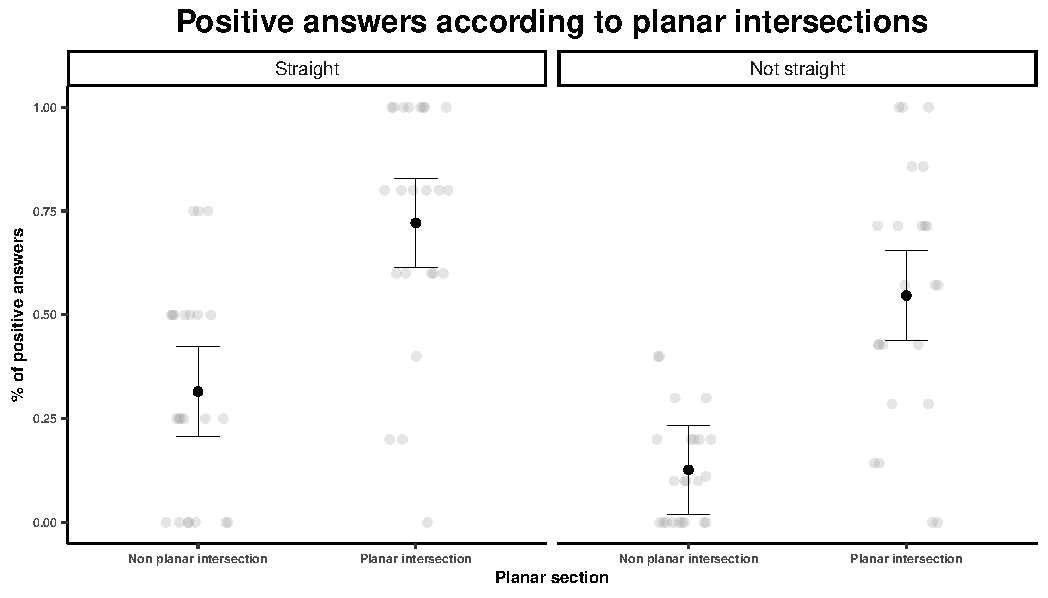
\includegraphics[scale=0.4]{group_straight.pdf}

          \end{centering}

          
          \footnotesize{N=23}
          
            Factor planar intersection: F(1,22)=53.32, p<.0001

          Factor straight: F(1,22)=19.09,  p=.0002

          No interaction 
          
        \footnotesize{Visually identical effects when putting random effect for each object, to ensure this is not due to accidental properties of shapes or lines}

        \end{frame}

        %% \begin{frame}


        %%               straight  1    6.39     p=.01, planar_intersection  1 17.78 ***  <.0001,  straight:planar_intersection  1      0.21     .65


        %%   \end{frame}

        \begin{frame}

          \begin{centering}
            
          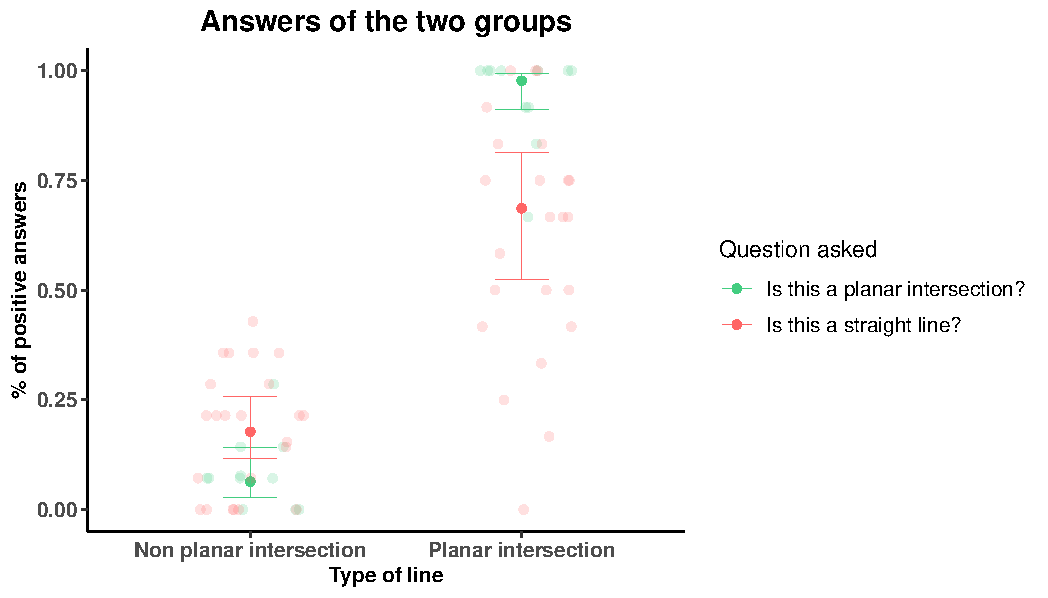
\includegraphics[scale=0.5]{two_groups.pdf}

          \end{centering}

          
          \footnotesize{
          group:  F(1,32)=2.28  p=.14}
          
          planar intersection: F(1,32)=213.60, p<.0001
          
          straight: F(1,32)=8.45, p=.007
          
          group x straight F(1,32)=6.94, p=.01


        \end{frame}



          
        %% \begin{frame}

        %%   Results synthesis

        %%   \begin{itemize}

        %%   \item{\textcolor{white}{First, the factor of planarity was strongly predictive of participants’ responses ( F(1,22)=53.32, p<.0001), even though it was orthogonal to straightness.}}

        %%   \item{\textcolor{white}{Second, when comparing pairs of (non-straight) curves matched for length and curvature, participants were more likely to identify planar intersections as straight lines (t(23)=5.14, p<.0001). }}

        %%   \item{\textcolor{white}{Third, participants’s answers were strongly correlated to the answers of another group of participants (N=11) asked to identify whether the lines were planar or not (r=0.81, p<.0001), which suggests that the two concepts coïncide. }}

        %%   \end{itemize}

          
        %% \end{frame}



        %% \begin{frame}

        %%   Results synthesis

        %%   \begin{itemize}

        %%   \item{First, the factor of planarity was strongly predictive of participants’ responses ( F(1,22)=53.32, p<.0001), even though it was orthogonal to straightness.}

        %%   \item{\textcolor{white}{Second, when comparing pairs of (non-straight) curves matched for length and curvature, participants were more likely to identify planar intersections as straight lines (t(23)=5.14, p<.0001). }}

        %%   \item{\textcolor{white}{Third, participants’s answers were strongly correlated to the answers of another group of participants (N=11) asked to identify whether the lines were planar or not (r=0.81, p<.0001), which suggests that the two concepts coïncide. }}

        %%   \end{itemize}
          
        %% \end{frame}

        
        %% \begin{frame}

        %%   Results synthesis

        %%   \begin{itemize}

        %%   \item{First, the factor of planarity was strongly predictive of participants’ responses ( F(1,22)=53.32, p<.0001), even though it was orthogonal to straightness.}

        %%   \item{Second, when comparing pairs of (non-straight) curves matched for length and curvature, participants were more likely to identify planar intersections as straight lines (t(23)=5.14, p<.0001). }

        %%   \item{\textcolor{white}{Third, participants answers were strongly correlated to the answers of another group of participants (N=11) asked to identify whether the lines were planar or not (r=0.81, p<.0001), which suggests that the two concepts coïncide. }}

        %%   \end{itemize}
          
        %% \end{frame}

        \begin{frame}

          Results synthesis

          \begin{itemize}

          \item{Factor of planarity strongly predictive of participants’ responses, transversaly to straightness }

          \item{Second, when comparing pairs of (non-straight) curves matched for length and curvature, participants were more likely to identify planar intersections as straight lines (t(23)=5.14, p<.0001). }

          \item{Third, participants’ answers were strongly correlated to the answers of another group of participants (N=11) asked to identify whether the lines were planar or not (r=0.81, p<.0001), which suggests that the two concepts coïncide. }

          \end{itemize}
          
        \end{frame}

        \begin{frame}

          How do this euclidean intuition evolve with mathematical education ?

           
           \end{frame}


        \begin{frame}

          How do this euclidean intuition evolve with mathematical education ?

          Two questions : 


          \begin{itemize}

          \item{When put in formal context, do participants reproduce this bias ? : Math educated participants (five years or more of formal education in maths, able to understand the exact definition of geodesic)}

           

          \item{Does the new concept collapses the former intuition or is there still traces of the planar heuristic ? Differential geometry experts (PhD or more in differential geometry or connex fields)}


           
           

            \end{itemize}

        \end{frame}




        
        
                    {
                      \setbeamercolor{background canvas}{bg=celadon}
                      \begin{frame}

                        \centering

                        Thanks for your attention !


                      \end{frame}
                    }
                    
\end{document}

